\documentclass[aspectratio=169]{beamer}

% Настройки темы из русского примера
\beamertemplatenavigationsymbolsempty
\usecolortheme{beaver}
\setbeamertemplate{blocks}[rounded=true, shadow=true]
\setbeamertemplate{footline}[page number]
\usefonttheme[onlymath]{serif}

% Пакеты
\usepackage[T2A]{fontenc}
\usepackage[utf8]{inputenc}
\usepackage[english,russian]{babel}
\usepackage{amssymb,amsfonts,amsmath,mathtext,mathtools}
\usepackage{subfig}
\usepackage[all]{xy}
\usepackage{array}
\usepackage{multicol}
\usepackage{hyperref}
\usepackage{hhline}
\usepackage{svg}
\usepackage{booktabs}
\usepackage{tabularx}
\usepackage{arydshln}
\usepackage{cleveref}
\usepackage{fontawesome5}
\usepackage{bm}

% Для наложения картинок на титульном слайде
\usepackage[absolute,overlay]{textpos}

% Настройка библиографии
\usepackage[style=authoryear, maxcitenames=1, maxbibnames=3, terseinits=true, uniquelist=false, natbib=true]{biblatex}
\addbibresource{solo_slides.bib} % Убедитесь, что файл рядом

% Beamer margin
\setbeamersize
{
    text margin left=0.5cm,
    text margin right=0.5cm
}

% Пути к картинкам
\graphicspath{{figs/}}

% --- ВАШИ ОПРЕДЕЛЕНИЯ МАТЕМАТИКИ ИЗ math_commands.tex И СЛАЙДОВ ---
\newcommand{\norm}[1]{\lVert #1\rVert}
\newcommand{\abs}[1]{\lvert #1 \rvert}
\renewcommand{\epsilon}{\varepsilon}
\newcommand{\R}{\mathbb{R}}
\newcommand{\Rmn}{\R^{m\times n}}
\newcommand{\cB}{\mathcal{B}}
\newcommand{\cS}{\mathcal{S}}
\newcommand{\cN}{\mathcal{N}}

\DeclarePairedDelimiter{\sqne}{\|}{\|_2^2}
\DeclarePairedDelimiter{\normf}{\|}{\|_\mathrm{F}}
\DeclarePairedDelimiter{\normkfk}{\|}{\|_\mathrm{KF-k}}
\DeclarePairedDelimiter{\normfstar}{\|}{\|_\mathrm{F*}}
\DeclarePairedDelimiter{\normftwo}{\|}{\|_\mathrm{F2}}
\DeclarePairedDelimiter{\sqns}{\|}{\|_{\mathrm{op}}^2}
\DeclarePairedDelimiter{\norms}{\|}{\|_{\mathrm{op}}}
\DeclarePairedDelimiter{\sqnn}{\|}{\|_{\mathrm{nuc}}^2}
\DeclarePairedDelimiter{\sqnf}{\|}{\|_{\mathrm{F}}^2}
\DeclarePairedDelimiter{\normn}{\|}{\|_{\mathrm{nuc}}}
\DeclarePairedDelimiter{\normfkfk}{\|}{\|_{\mathrm{F-KF-k}}}
\def\<#1,#2>{\langle #1,#2\rangle}
\DeclarePairedDelimiter{\dotprod}{\langle}{\rangle}

\DeclareMathOperator{\tr}{tr}
\DeclareMathOperator{\diag}{diag}
\DeclareMathOperator*{\argmin}{arg\,min}
\DeclareMathOperator*{\Argmin}{Arg\,min}
\DeclareMathOperator*{\argmax}{arg\,max}
\DeclareMathOperator*{\Argmax}{Arg\,max}
\DeclareMathOperator{\sign}{sign}

% Векторы и матрицы (жирный шрифт)
\def\vu{{\bm{u}}}
\def\ve{{\bm{e}}}
\def\vv{{\bm{v}}}
\def\mM{{\bm{M}}}
\def\mX{{\bm{X}}}
\def\mU{{\bm{U}}}
\def\mV{{\bm{V}}}
\def\mD{{\bm{D}}}
\def\mN{{\bm{N}}}
\def\mSigma{{\bm{\Sigma}}}
% -----------------------------------------------------------------

%----------------------------------------------------------------------------------------------------------
\title[Неспектральные матричные нормы]{Неспектральные матричные нормы для обучения нейронных сетей}

\author[А.\,Ю.~Кравацкий]{Алексей Юрьевич Кравацкий\\
\small{Научный руководитель: д.ф.-м.н., проф. РАН И.\,В.~Оселедец}}

\institute{Кафедра интеллектуальных систем ФПМИ МФТИ\\
Специализация: Интеллектуальный анализ данных\\
Направление: 03.03.01 Прикладные математика и физика}
\date{2026}


\begin{document}

\begin{frame}[plain]
  \maketitle
  % Картинки на титульном слайде
  \begin{textblock*}{0.2\paperwidth}(0.77\paperwidth,0.6\paperheight)
    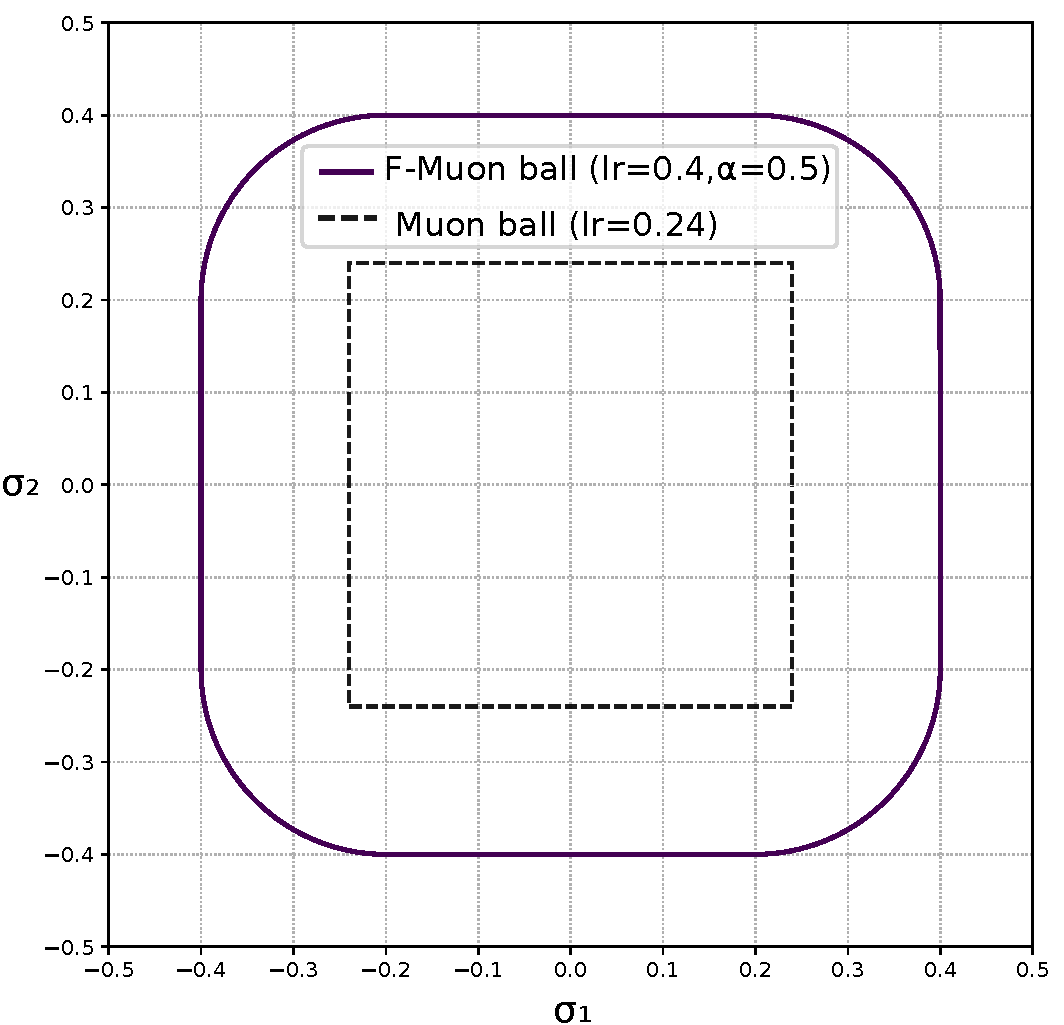
\includegraphics[width=\linewidth]{norms/fstardual_cifar.pdf}
  \end{textblock*}
  \begin{textblock*}{0.22\paperwidth}(0.03\paperwidth,0.55\paperheight)
    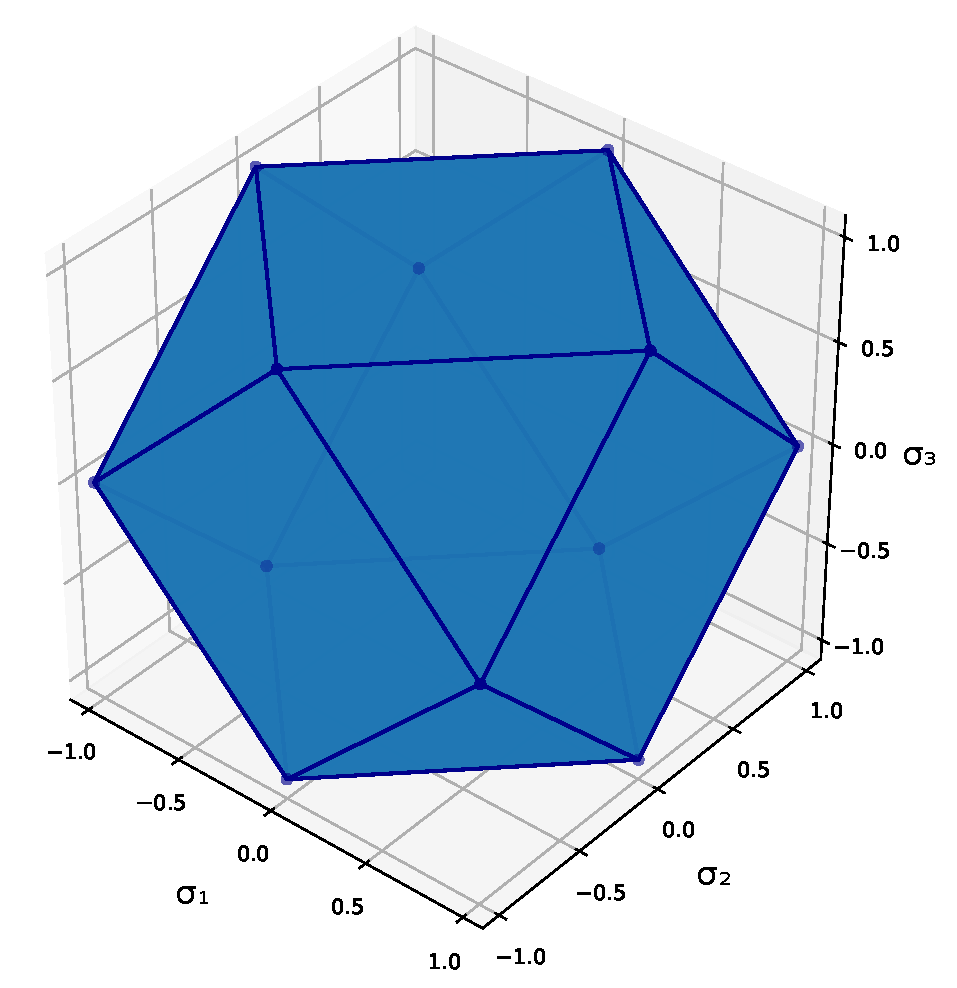
\includegraphics[width=\linewidth]{norms/KyFanDual.pdf}
  \end{textblock*}
\end{frame}

%------------------------------------------------------------------------------------
\begin{frame}{Неспектральные матричные нормы для обучения нейронных сетей}
    \begin{block}{Проблема}
        Поиск $\argmin_{\mX\in\R^{m\times n}} f(\mX)$, в особенности когда $\mX$ — матрица весов в нейронной сети
    \end{block}

    \begin{block}{Цель}
        В рамках подхода norm-constrained linear minimization oracle (LMO) \citep{pethick2025training} отойти от спектральной нормы, чтобы получить эффективные алгоритмы для обучения внутренних слоёв нейросети взамен Muon.
    \end{block}

    \begin{block}{Решение}
        На основе норм Ки Фана предлагается построить матричные нормы, порождающие семейства алгоритмов \emph{Fanions}, связанные с Muon, $\nu$-SAM и Dion, а также \emph{F-Fanions} и \emph{S-Fanions}, объединяющие Fanions с Normalized SGD (NSGD) и SignSGD.
    \end{block}
\end{frame}

%-------------------------------------------------------------------------------------
\begin{frame}{Norm-constrained LMO: задача выбора нормы}
  Наделим пространство $\Rmn$ нормой $\norm{\cdot}$ с единичным шаром $\cB_1 = \{ \mD \in \Rmn \mid \norm{\mD} \le 1 \}$. Её двойственная норма определяется как $\norm{\mM}^\dagger = \sup_{\mD \in \cB_1} \<\mM,\mD>$.

  \vspace{0.4em}

  Направление $\mathrm{LMO}(\mM^t) \in \Argmin_{\mD \in \cB_1} \langle\mM^t, \mD\rangle$, где $\mM^t$ — градиент или моментум, задаёт обновление:
  \[
  \begin{aligned}
    \mX^{t+1} &= \mX^{t} + \gamma_t \, \mathrm{LMO}(\mM^t) \in \mX^{t} - \gamma_t \Argmax_{\mD \in \cB_1} \langle \mM^t, \mD \rangle \\
    &= \mX^{t} - \gamma_t \{\Delta \in \cB_1 \mid \langle \mM^t, \Delta \rangle = \norm{\mM^t}^\dagger\}.
    \end{aligned}
  \]
  \begin{block}{Рецепт}
     Надо найти направление $\Delta \in \cB_1$, которое доставляет равенство $\<\mM^t, \Delta> = \norm{\mM^t}^\dagger$. Для этого часто требуется SVD разложение: $\mM^t = \mU \mSigma \mV^\top = \mU \diag(\sigma_1, \dots, \sigma_r) \mV^\top$.
  \end{block}

  \begin{block}{Требуется}
    Выяснить, какие $\norm{\cdot}$, помимо спектральной $\norms{\cdot}$, задают эффективные на практике алгоритмы.
 \end{block}
\end{frame}
%-------------------------------------------------------------------------------------
\begin{frame}{LMO-алгоритмы в нормах Шаттена $S_p$ и векторных $l_p$ нормах}
  \footnotesize
  \begin{table}
  \label{tbl:mat_vs_vec_lmo}
  \begin{tabularx}{\linewidth}{|>{\raggedright\arraybackslash}X|c|c|c|}
  \hline
  Метод & $\norm{\cdot}$ для LMO & Обновление LMO & Ссылка \\
  \hline\hline
  Normalized SGD & Евклидова $l_2$ / & $-\gamma_t \tfrac{g}{\norm{g}_2} = -\gamma_t \tfrac{g}{\norm{g}_F}$ & \citep{hazan2015beyond} \\
  Momentum Normalized SGD & Фробениусова $S_2$ & $-\gamma_t \tfrac{g}{\norm{g}_2} = -\gamma_t\tfrac{g}{\norm{g}_F}$ & \citep{cutkosky2020momentum}\\
  \hline
  SignSGD & $l_\infty$ (Max-норма) & $-\gamma_t \sign(g)$ & \citep{bernstein2018signsgd} \\
  Signum  & $l_\infty$ (Max-норма) & $-\gamma_t \sign(g)$ & \citep{bernstein2018signsgd} \\
  \hdashline
  Muon & Спектральная $S_\infty$ & $-\gamma_t \mU\mV^\top$ & \citep{jordan2024muon} \\
  \hline
  Gauss-Southwell Descent & Шар в $l_1$ & $-\gamma_t \sum_{i \in \argmax|g_i^t|} \sign(g_i^t)\ve_i$ & \citep{shi2016primer}\\
  \hdashline 
  Neon & Ядерная $S_1$ & $-\gamma_t \vu_1 \vv_1^\top$ & \citep{kravatskiy2025fanions} \\
  $\nu$SAM & Ядерная $S_1$ &  & \citep{pethick2025sam} \\
  \hline
  \end{tabularx}
  \end{table}
\end{frame}
%-------------------------------------------------------------------------------------
\begin{frame}{Проблема ранга LMO-обновлений}
  Нормы Шаттена $\norm{\mM^t}_{S_p} = \left(\sum_{i=1}^{\min(m, n)}\sigma_i^p\right)^{1/p}\,$ дают шаг обновления
  \[
  \mX^{t+1} = \mX^t - \gamma_t \mU \frac{\diag\left(\sigma_1^{q-1},\dots, \sigma_{\min(m,n)}^{q-1}\right)}{\left(\sum_{i=1}^{\min(m,n)}{\sigma_i^q}\right)^{\frac{q-1}{q}}}\mV^\top
  \]
  где $p^{-1} + q^{-1} = 1$ \citep{cesista2025schattenp}.

  \vspace{0.5em}
  Нормы Ки Фана $\normkfk{\mM^t}= \sum_{i=1}^{k}\sigma_i\,$ дают 
  \[
  \mX^{t+1} = \mX^{t} - \gamma_t \vu_1 \vv_1^\top\text{ \quad или \quad }\mX^{t+1} = \mX^{t} - \frac{\gamma_t}{k}\mU \mV^\top\,,
  \]
  что соответствует алгоритмам Neon или Muon \citep{kravatskiy2025fanions}.

  \vspace{0.5em}
  \alert{Следствие:} обновления получаются либо одноранговыми, либо полноранговыми.
\end{frame}

%----------------------------------------------------------------------------------------------------------
\begin{frame}{Нормы $\normkfk{\cdot}^\dagger$, двойственные к нормам Ки Фана, и алгоритмы Fanions}
  Пусть $\norm{\cdot} = \normkfk{\cdot}^\dagger$. Возьмём направление $\Delta = \sum_{i=1}^k{\vu_i \vv_i^\top}$. Его норма $\normkfk{\Delta}^\dagger = \max\{\frac{1}{k} \normn{\Delta}, \norms{\Delta}\} = \max\{\frac{1}{k} k, 1\} = 1$, и скалярное произведение 
  \[
  \begin{aligned}
  \<\mM^t, \Delta> &=\<\mU \mSigma \mV^\top, \sum_{i=1}^{k} \vu_i \vv_i^\top> = \sum_{i,j=1}^{r, k}\<\vu_i \sigma_i \vv_i^\top, \vu_j \vv_j^\top> = \sum_{i=1}^{k}\sigma_i \\
  &= \normkfk{\mM^t} = \normkfk{\mM^t}^{\dagger\dagger} = \norm{\mM^t}^\dagger.
  \end{aligned}
  \]  
  Следовательно, искомое обновление для Fanion-$k$ принимает вид:
  $$\mX^{t+1} = \mX^{t} - \gamma_t \sum_{i=1}^{k} \vu_i \vv_i^\top$$
\end{frame}

%-----------------------------------------------------------------------------------------------------------
\begin{frame}{Ограничения на сингулярные числа в LMO с нормами Ки Фана и двойственными к ним}
\centering
\begin{minipage}{0.46\textwidth}
    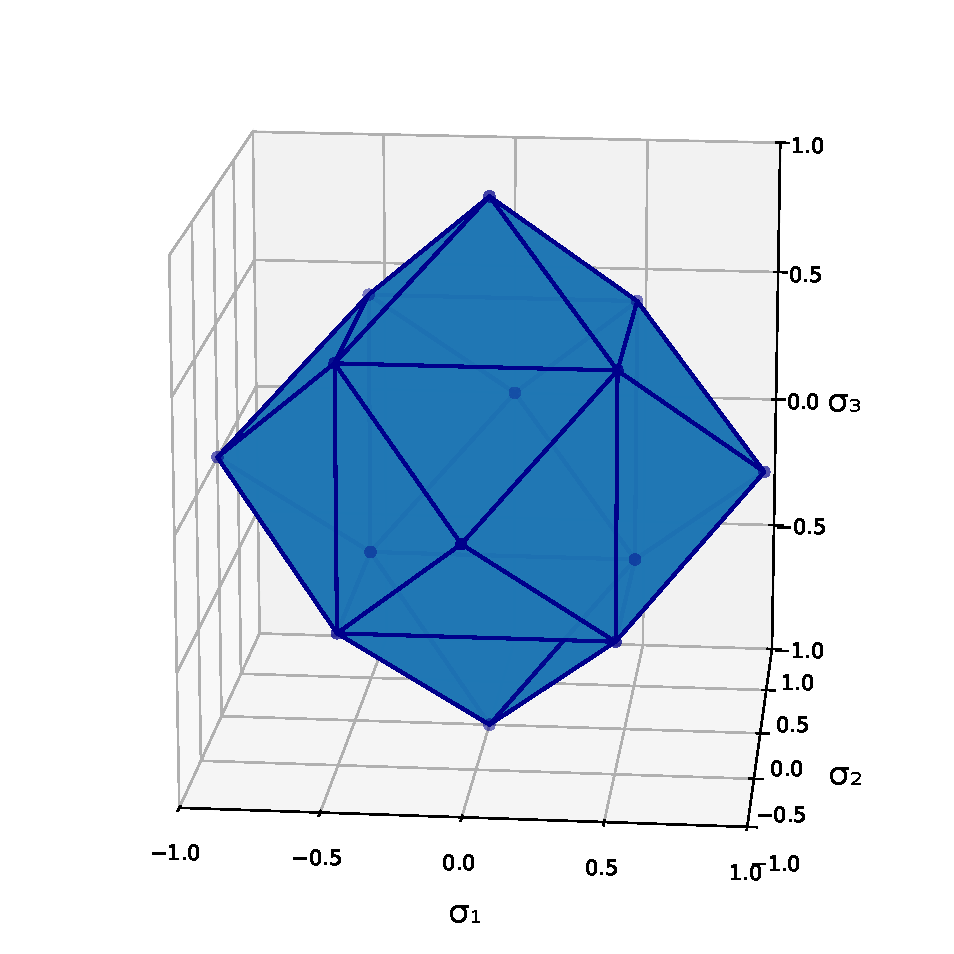
\includegraphics[height=0.75\textheight,keepaspectratio]{norms/KyFan.pdf}
\end{minipage}\hfill
\begin{minipage}{0.46\textwidth}
    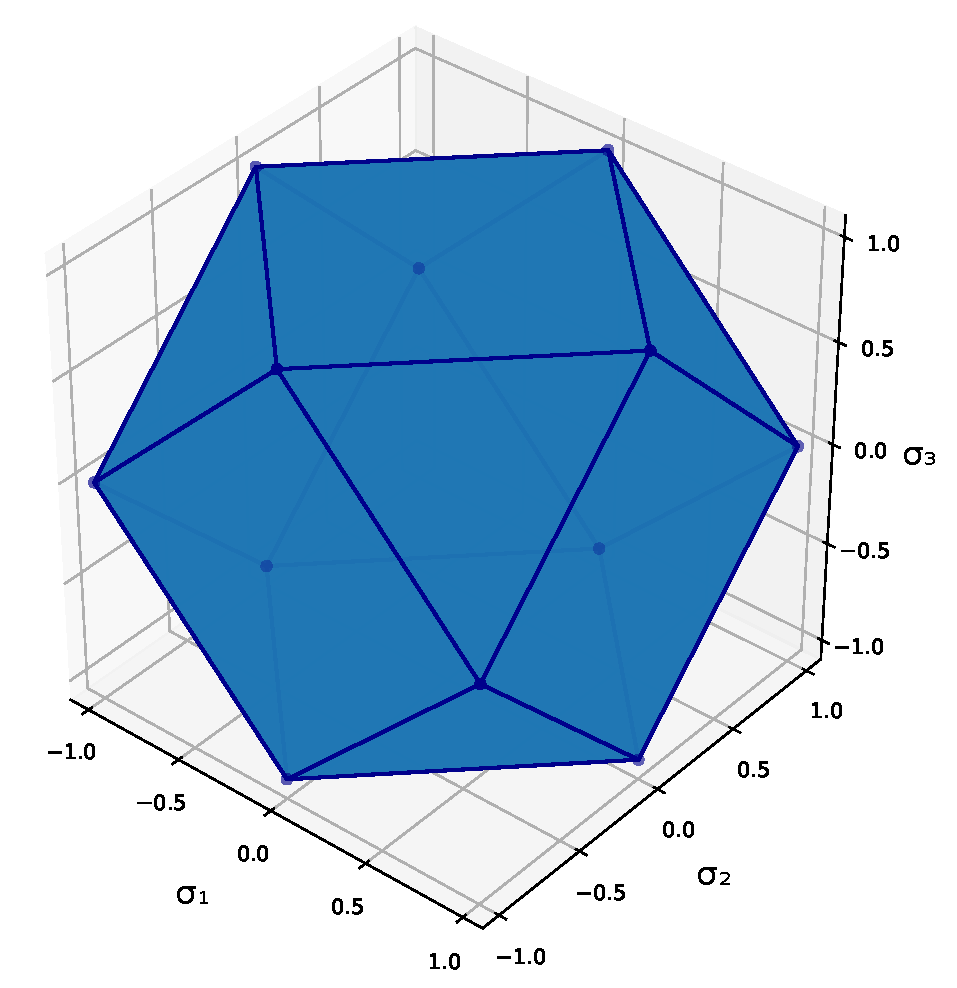
\includegraphics[height=0.75\textheight,keepaspectratio]{norms/KyFanDual.pdf}
\end{minipage}

\vspace{0.3em}
\footnotesize $\cB_1$ для нормы Ки Фана ранга $k=2$ и для двойственной к ней норме $\normkfk{\cdot}^\dagger = \max\left\{\frac{1}{k} \normn{\cdot}, \norms{\cdot}\right\}\,$ .
\end{frame}

% %--------------------------------------------------------------------------------------------------------------
% \begin{frame}{Двойственные шары для выпуклых комбинаций норм}
%   \begin{block}{Лемма 1 \citep{yu2012arithmetic}}
%     Пусть $\norm{\cdot}_{(1)},\dots,\norm{\cdot}_{(n)}$ — нормы в конечномерном евклидовом пространстве, а $\alpha_1,\dots,\alpha_n$ — неотрицательные числа. Определим
%     \[
%       \norm{\cdot} := \sum_{i = 1}^n \alpha_i \norm{\cdot}_{(i)}\,.
%     \]
%     Тогда единичный шар двойственной нормы $\norm{\cdot}^\dagger$ удовлетворяет
%     \[
%       \cB_{\norm{\cdot}^\dagger}
%       = \sum_{i = 1}^n \alpha_i \cB_{\norm{\cdot}_{(i)}^\dagger}\,,
%     \]
%     где $\sum$ обозначает сумму Минковского, а $\cB_{\norm{\cdot}_{(i)}^\dagger}$ — единичный шар двойственной нормы $\norm{\cdot}_{(i)}^\dagger$.
%   \end{block}
% \end{frame}

%--------------------------------------------------------------------------------------------------------------
\begin{frame}{Коническая комбинация LMO}
    \begin{block}{Лемма (Кравацкий, 2025)}
      Пусть задано конечное семейство LMO-алгоритмов $i = 1,\dots,n$, где обновление $i$-го алгоритма на шаге $t$ определяется как
      \[
      \mX^{t + 1} - \mX^{t} = \gamma_t \mathrm{LMO}_{\norm{\cdot}_{(i)}}(\mM^{t})\,,
      \]
      и $\mathrm{LMO}_{\norm{\cdot}_{(i)}}$ соответствует единичному шару нормы $\norm{\cdot}_{(i)}$.
      
      Тогда для любых неотрицательных $\alpha_1,\dots,\alpha_n$, алгоритм с обновлением
      \[
      \mX^{t + 1} - \mX^{t} = \gamma_t \sum_{i = 1}^n \alpha_i \mathrm{LMO}_{\norm{\cdot}_{(i)}}(\mM^t)
      \]
      сам является LMO-алгоритмом, соответствующим единичному шару нормы, двойственной к норме $\sum_{i = 1}^n \alpha_i \norm{\cdot}_{(i)}^\dagger$.
    \end{block}
\end{frame}

% %-------------------------------------------------------------------------------------
% \begin{frame}{За пределами спектральной нормы и Muon}

%   От спектральной нормы $\norms{\cdot}$ и алгоритма Muon:
%   $$\mX^{t+1} = \mX^{t} - \gamma_t \mU \mV^\top$$
%   К двойственной норме $\normkfk{\cdot}^\dagger$ и общему алгоритму F-Fanion:
%   $$\mX^{t+1} = \mX^{t} - \gamma_t \left(\alpha \sum_{i=1}^k{\vu_i \vv_i^\top} + (1-\alpha)\frac{\mM^t}{\normf{\mM^t}}\right), \quad \alpha \in [0,1]$$
%   И к общему алгоритму S-Fanion (на базе нормы $\norm{\cdot}^\dagger_{\mathrm{C^\dagger-KF-k}}$):
%   $$\mX^{t+1} = \mX^{t} - \gamma_t \left(\alpha \sum_{i = 1}^k \vu_i \vv_i^\top + (1-\alpha)\gamma_t\sign(\mM^t)\right), \quad \alpha \in [0,1], \gamma_t > 0$$
% \end{frame}

%-----------------------------------------------------------------------------------------------------------
\begin{frame}{Гибридные алгоритмы: F-Fanions и S-Fanions}

  $\alpha \times$Fanion (норма $\normkfk{\cdot}^\dagger$) + $(1-\alpha) \times$NSGD (норма $\normf{\cdot}$) \textbf{= F-Fanion}:
  $$\mX^{t+1} = \mX^{t} - \gamma_t \left(\alpha \sum_{i=1}^k{\vu_i \vv_i^\top} + (1-\alpha)\frac{\mM^t}{\normf{\mM^t}}\right)$$

  \vspace{0.5em}
  $\alpha \times$Fanion + $(1-\alpha)\times\eta\times$SignSGD (норма $\eta||\cdot||_\infty$) \textbf{= S-Fanion}:  

  $$\mX^{t+1} = \mX^{t} - \gamma_t \left(\alpha \sum_{i = 1}^k \vu_i \vv_i^\top + (1-\alpha)\eta\sign(\mM^t)\right)$$

\end{frame}

%---------------------------------------------------
\begin{frame}{Число итераций до $F(\mX)\leq0.001$ для гладкой выпуклой $F$}
  \begin{columns}[T,totalwidth=\textwidth]
    \begin{column}{0.48\textwidth}
      
\includegraphics[width=\linewidth]{simple_lls/loss_long_run_16_increase.pdf}
      \centering
      \scriptsize $F(\mX)$
    \end{column}
    \begin{column}{0.48\textwidth}
      
\includegraphics[width=\linewidth]{simple_lls/gradient_frobenius_norm_vs_iteration_long_run.pdf}
      \centering
      \scriptsize $\normf{\nabla F(\mX)}$
    \end{column}
  \end{columns}
  \vspace{0.3em}
  \centering
  \footnotesize Задача: $F(\mX) = \frac{1}{2}\normf{\mM^{1/2}\mX\mN^{1/2}}^2 \to \min_{\mX \in \R^{500\times 500}}\,$, где $\lambda(\mM), \lambda(\mN) \sim U[0,1]$, $\mX^0_{ij} \sim \cN(0,1)$.
\end{frame}

%---------------------------------------
\begin{frame}{Обучение CNN: CIFAR-10 airbench}
  \begin{columns}[T,totalwidth=\textwidth]
    \begin{column}{0.48\textwidth}
      
\includegraphics[width=\linewidth]{cifar_logger/train_acc.pdf}
      \centering
      \scriptsize Точность на обучающей выборке
    \end{column}
    \begin{column}{0.48\textwidth}
      
\includegraphics[width=\linewidth]{cifar_logger/val_acc.pdf}
      \centering
      \scriptsize Точность на валидационной выборке
    \end{column}
  \end{columns}
\end{frame}
%-----------------------------------------
\begin{frame}{Нормы стохастических градиентов (layer2.conv2, CIFAR-10 airbench)}
  \begin{columns}[T,totalwidth=\textwidth]
    \begin{column}{0.48\textwidth}
      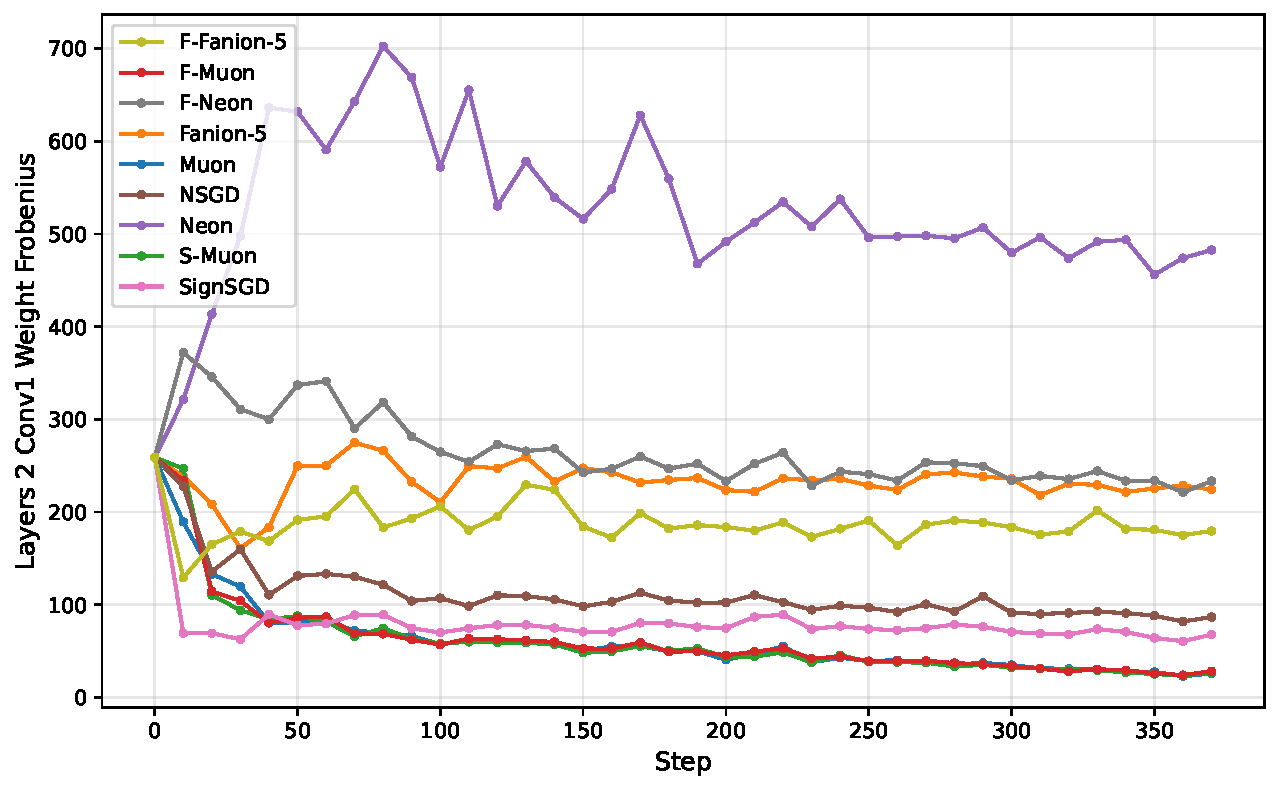
\includegraphics[width=\linewidth]{cifar_logger/layers_2_conv1_weight_frobenius.pdf}
      \centering
      \scriptsize Норма Фробениуса
    \end{column}
    \begin{column}{0.48\textwidth}
      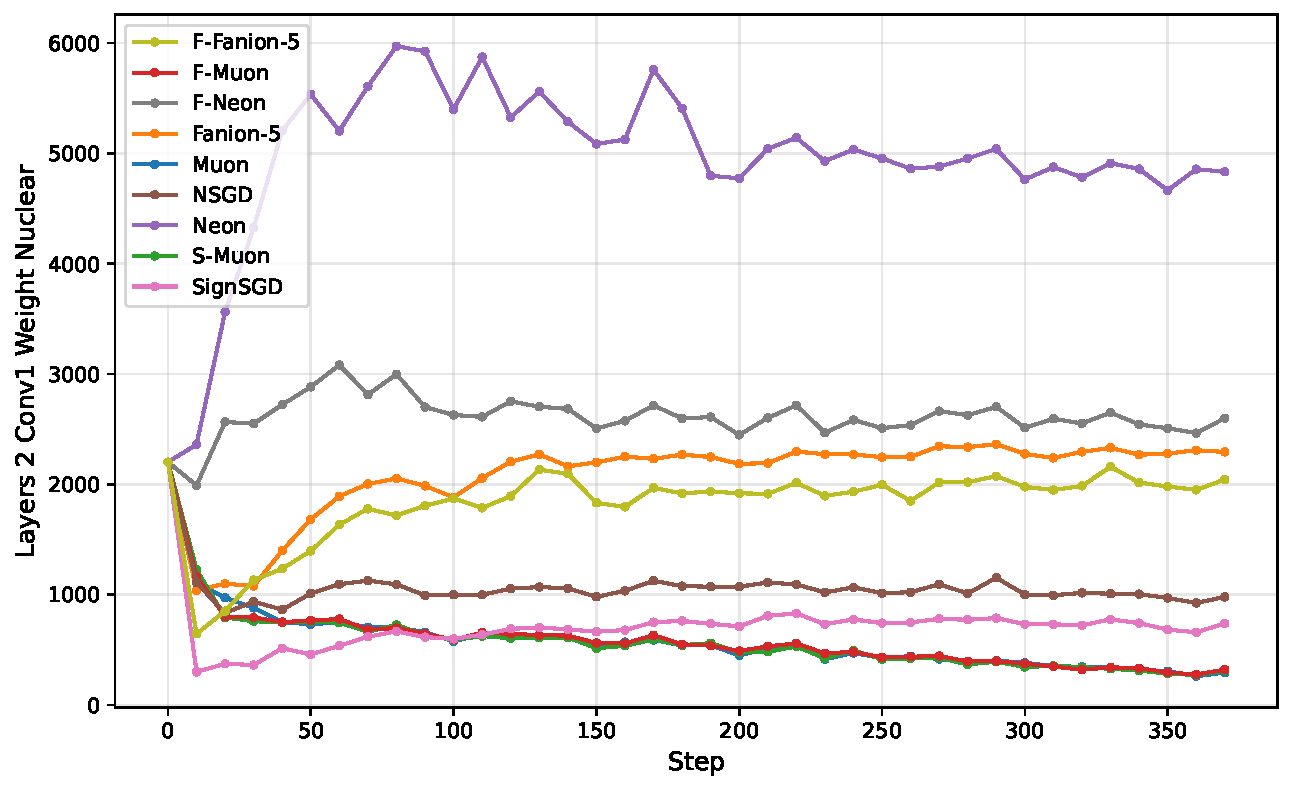
\includegraphics[width=\linewidth]{cifar_logger/layers_2_conv1_weight_nuclear.pdf}
      \centering
      \scriptsize Ядерная норма
    \end{column}
  \end{columns}
\end{frame}
%----------------------------------------
\begin{frame}{LMO-шары алгоритмов на CIFAR-10 airbench}
  \begin{figure}[t]
    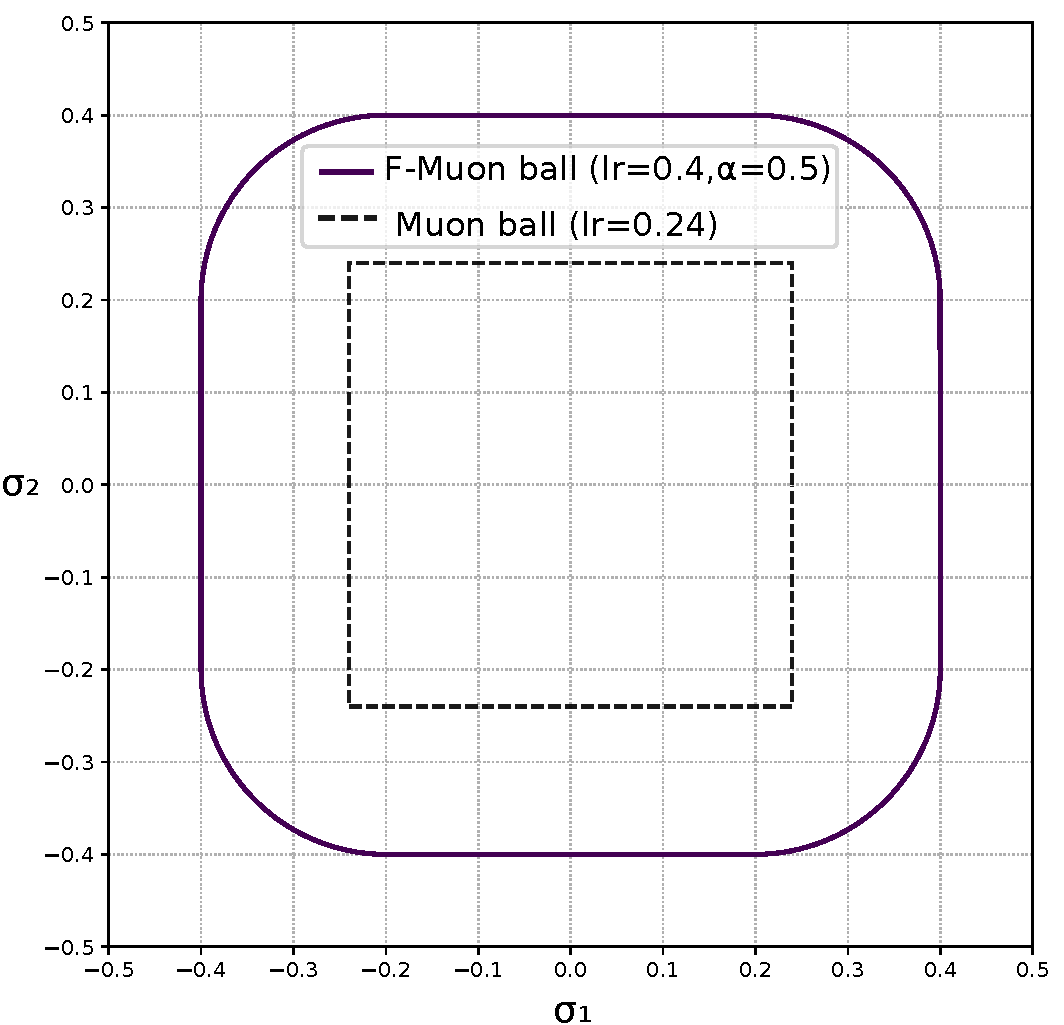
\includegraphics[height=0.65\textheight]{norms/fstardual_cifar.pdf}
    \centering
    
    \vspace{0.2em}
    \footnotesize $\cB_{\texttt{learning\_rate}}$ для норм, порождающих Muon и F-Muon
  \end{figure}
\end{frame}

%--------------------------------------------
\begin{frame}{F-Muon на CIFAR-10 airbench: зависимость от $\alpha$}
    \begin{columns}[T,totalwidth=\textwidth]
      \begin{column}{0.48\textwidth}
        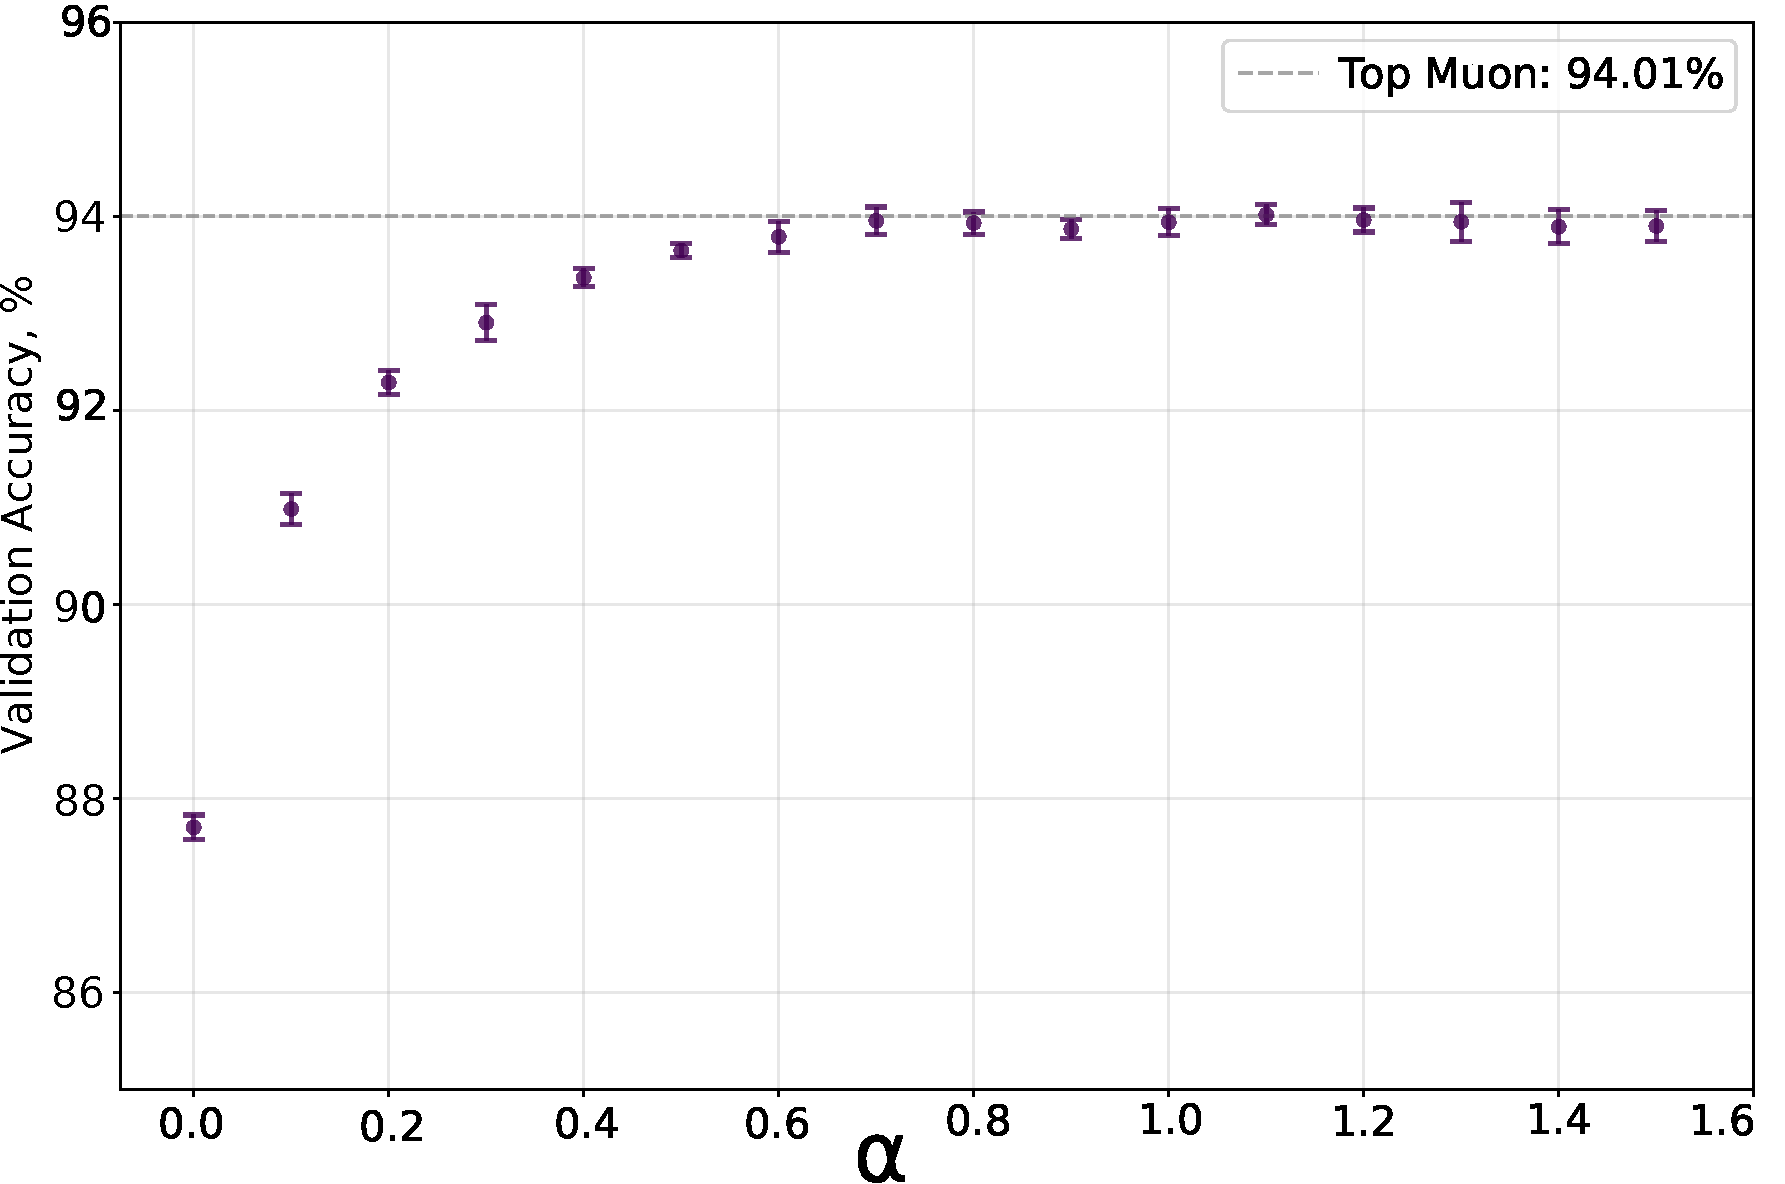
\includegraphics[width=\linewidth]{muon_tuned_diff_alpha.pdf}
        \centering
        \scriptsize Гиперпараметры оптимальны для Muon \citep{cifar2023airbench}
      \end{column}
      \begin{column}{0.48\textwidth}
        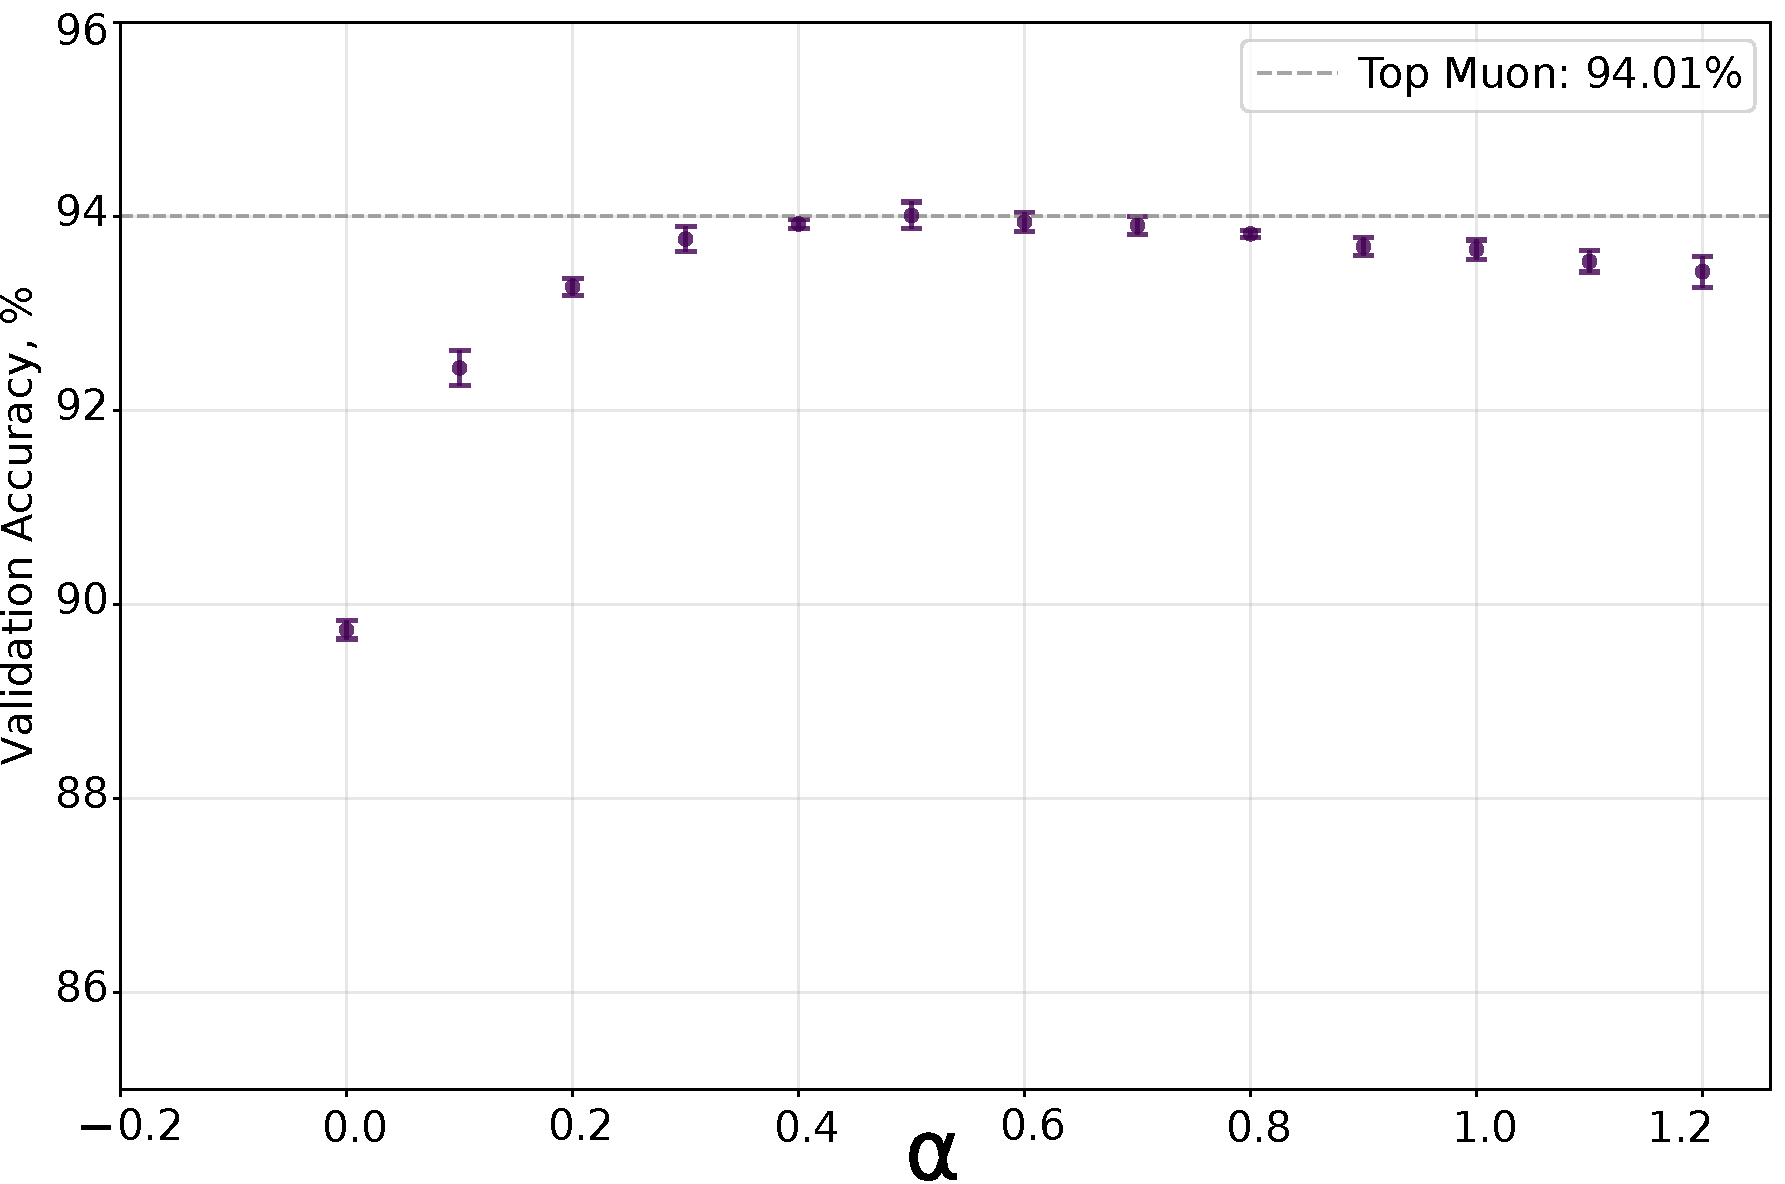
\includegraphics[width=\linewidth]{fmuon_tuned_diff_alpha.pdf}
        \centering
        \scriptsize Гиперпараметры оптимальны для F-Muon с $\alpha=0.5$
      \end{column}
    \end{columns}
    \vspace{0.6em}
    \centering

    \faExclamationCircle \space F-Fanion с параметром $\alpha > 1$ \textbf{не является} LMO-алгоритмом.
\end{frame}
%-----------------------------------------
\begin{frame}{Предобучение NanoGPT и GPT-2 Medium на FineWeb}
  \begin{columns}[T,totalwidth=\textwidth]
    \begin{column}{0.48\textwidth}
      
\includegraphics[width=\linewidth]{nanogpt/nano/val_loss_vs_step.pdf}
      \centering
      \scriptsize Модель NanoGPT
    \end{column}
    \begin{column}{0.48\textwidth}
      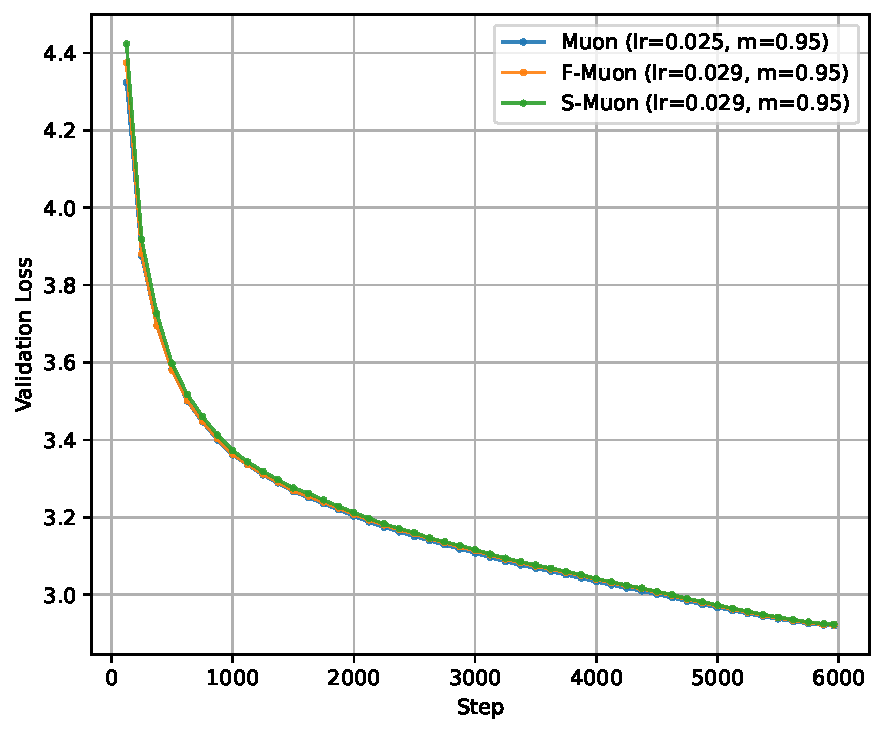
\includegraphics[width=\linewidth]{nanogpt/medium/val_loss_vs_step.pdf}
      \centering
      \scriptsize Модель GPT-2 Medium
    \end{column}
  \end{columns}
\end{frame}

%----------------------------------------
\begin{frame}{Выносится на защиту}
    \begin{enumerate}
        \item Обобщение алгоритма Muon до семейства алгоритмов Fanions на основе норм, двойственных к нормам Ки Фана
        \item Лемма о том, что коническая комбинация LMO-алгоритмов является LMO-алгоритмом
        \item Гибридные семейства алгоритмов F-Fanions и S-Fanions, объединяющие обновление Fanions с Normalized SGD и SignSGD
        \item Показано, что F-Muon и S-Muon сопоставимы с Muon на задачах обучения свётрочных сетей (CIFAR-10 airbench) и трансформеров (NanoGPT, GPT-2).
    \end{enumerate}
    \begin{block}{Список работ автора по теме ВКР}
        \begin{enumerate}
        \item \textbf{Kravatskiy A.} et al. The Ky Fan Norms and Beyond: Dual Norms and Combinations for Matrix Optimization // \emph{International Conference on Computational Optimization}, 2025 \& \emph{Special Issue: Computational Optimization for Machine Learning and Data Science} в \emph{Journal of Optimization Theory and Applications} (Q1) (на рецензировании)
        
        \end{enumerate}
    \end{block}
\end{frame}

%----------------------------------------
\begin{frame}[allowframebreaks]{Список литературы}
  \printbibliography
\end{frame}

\end{document}